%%%%% Document Setup %%%%%%%%

\documentclass[12pt, onecolumn]{revtex4}    % Font size (12pt) and column number (one or two).

\usepackage[a4paper, left=2.5cm, right=2.5cm, top=2.5cm, bottom=2.5cm]{geometry}  % Defines paper size and margin length

\renewcommand{\baselinestretch}{1}     % Defines the line spacing

\usepackage{subcaption}

\usepackage[font=small, labelfont=bf]{caption}                      % Defines caption font size and caption title bolded
\captionsetup[figure]{justification=justified, singlelinecheck=off, font=footnotesize} 
\captionsetup{compatibility=false}

\usepackage{graphics,graphicx,epsfig,ulem}	% Makes sure all graphics works
\usepackage{amsmath} 						% Adds mathematical features for equations

\usepackage{etoolbox}                       % Customise date to preferred format
\makeatletter
\patchcmd{\frontmatter@RRAP@format}{(}{}{}{}
\patchcmd{\frontmatter@RRAP@format}{)}{}{}{}
\renewcommand\Dated@name{}
\makeatother

\usepackage[UKenglish]{babel}% http://ctan.org/pkg/babel

\usepackage{fancyhdr}

\pagestyle{fancy}                           % Insert header
\renewcommand{\headrulewidth}{0pt}
\lhead{\small Z0962251}  

\def\thesection{\arabic{section}}
\def\thesubsection{\alph{subsection}}

\def\bibsection{\section*{References}}        % Position reference section correctly
\setcitestyle{authoryear,round}
\setlength\bibhang{0.2in}
\usepackage[colorlinks]{hyperref}
\hypersetup{
    colorlinks=true,
    linkcolor=black,
    citecolor=black,    
    urlcolor=black,
}

%%%%% Document %%%%%
\begin{document}                     


\title{The measurement of the Hubble Constant: beyond the cosmic ladder} 
\date{Submitted: \today{}}
\author{Z0962251}

\maketitle
\thispagestyle{plain} % produces page number for front page

% Introduction to Hubble's constant and it's importance
A precisely determined Hubble's constant $H_0$ would have an overarching effect on any feature of cosmological theory: the age or critical density of the Universe, or with the formation of cosmic structure. Producing a conclusive value for $H_0$ is difficult as absolute distances on the cosmic scale are difficult to measure. Inhomogeneous gravitational acceleration generates motion which does not follow the simple expansion as described by Hubble's Law $v=H_0 d$. An uncertainty arises due to the discrepancy between the methods to connect local distances to the smooth large-scale Hubble flow \citep{fukugita_cosmic}. \\
% words: 88

% Cosmic distance ladder and cosmic paths
Several approaches for cosmic distance measurement should therefore be used to reduce systematic errors. These measurements can form the ``rungs'' of a \textit{cosmic distance ladder}, where large extragalactic distances ($>1000$ Mpc) are informed and calibrated by techniques which have smaller ranges \citep{carroll_astro}. Astronomers may employ a variety of methods in tandem, therefore the ladder could instead be expressed as several pathways (Figure \ref{fig:cosmic_pathways}). 
% words: 63

% reiterate somewhere that galaxies should be distant so their peculiar velocities are small compared to the hubble flow

\begin{center}
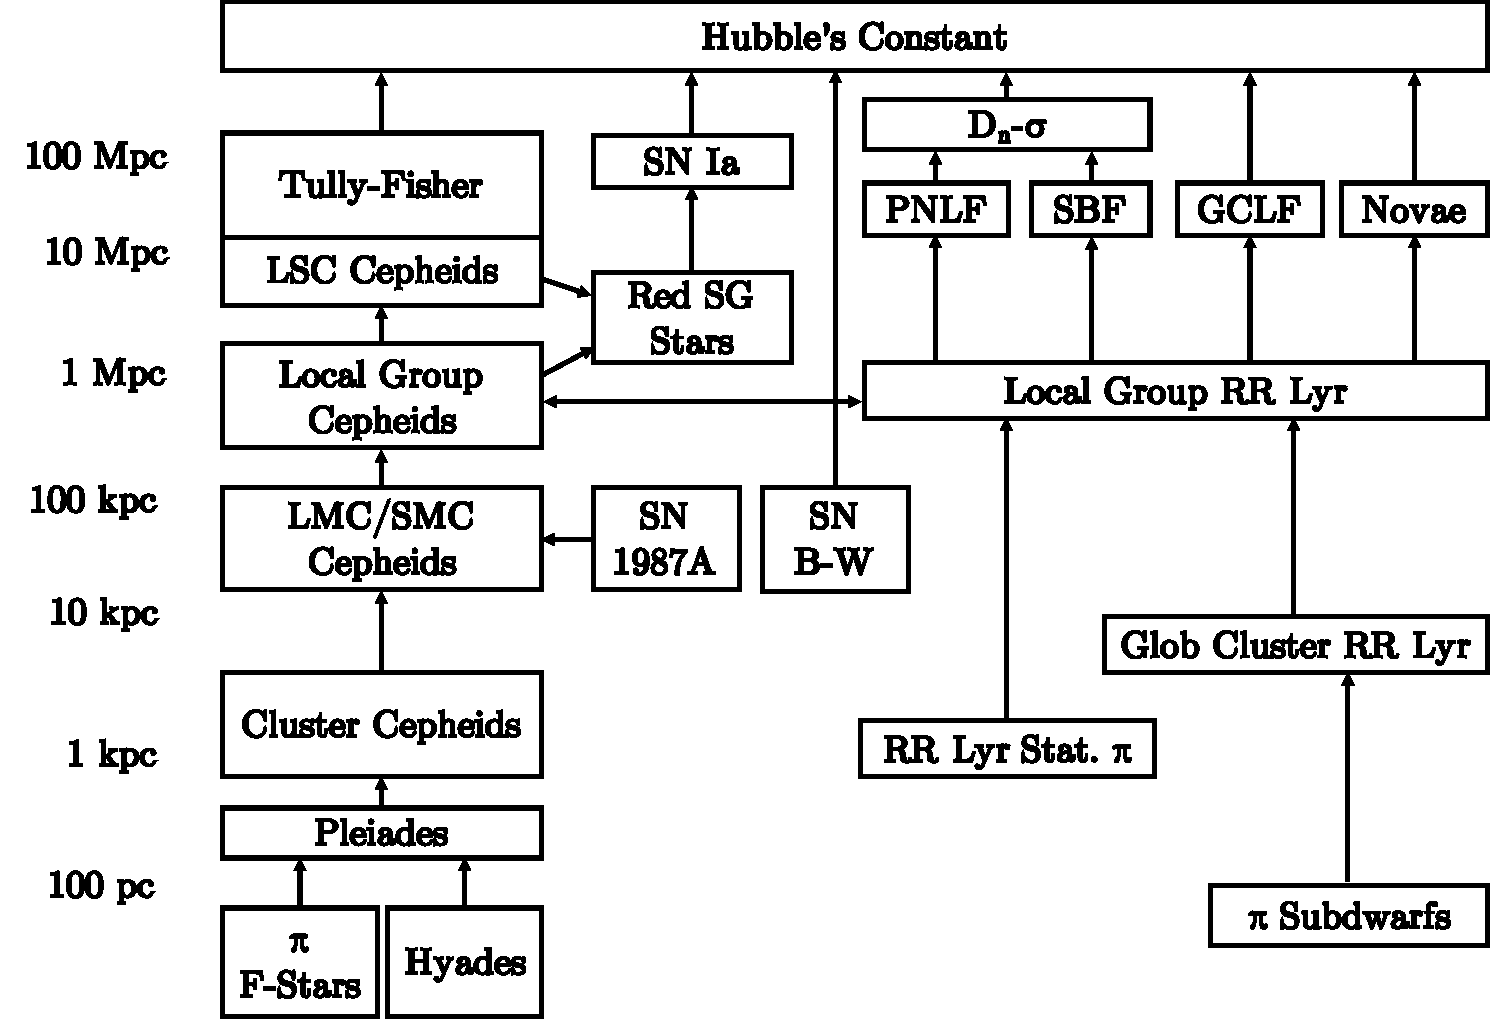
\includegraphics[width=0.8\linewidth]{figures/cosmic_distance_pathways}
\captionof{figure}[Cosmic Distance Pathways]{Adapted from \cite{jacoby_extragal}, this diagram illustrates the various approaches to calculate $H_0$, each technique is roughly placed at the approximate range it operates at. One can see that there is not one strict ``cosmic ladder'', rather multiple pathways. For reference, the acronyms used are: B-W - Baade-Wessenlink; GCLF - Globular-Cluster Luminosity Function; LSC - Local Super Cluster; PNLF - Planetary Nebula Luminosity Function; SBF - Surface-Brightness Fluctuations; SG - Super Giant; SN - Supernovae; $\pi$ - parallax.}
\label{fig:cosmic_pathways}
\end{center}

% HST Key Project
The Hubble Space Telescope (HST) $H_0$ Key Project was an effort in the early 2000s to determine $H_0$ by calculating distances to Cepheid variables in local galaxies ($\le 20$ Mpc) then applying them as a calibration to 5 secondary independent distance indicators. Described by \cite{freedman_hstkeystone}, four of the methods (Type Ia supernovae, Tully-Fisher relation, surface-brightness fluctuations, and Type II supernovae) were able to produce $70\le H_0 \le72$ kms$^{-1}$ Mpc$^{-1}$ and the remaining technique (fundamental plane for elliptical galaxies) $H_0\approx82$ kms$^{-1}$ Mpc$^{-1}$. Over the next decade, the methodology would be refined and the sample of Cepheids and Type Ia supernovae improved (better observations and other data types) $H_0=73.48 \pm1.66$ kms$^{-1}$ Mpc$^{-1}$ \citep{2011ApJ...730..119R, 2016ApJ...826...56R, 2018ApJ...855..136R}. These results set a standard benchmark for $H_0$, they were found by taking steps along the cosmic ladder and whilst they have high accuracy, it would be beneficial to directly calculate $H_0$ at large distances without the need for Cepheid-based calibration. \\
% words: 144

% CMB anisotropies, Planck
One alternative is measuring Cosmic Microwave Background (CMB) anisotropies. Through analysing all-sky temperature and polarisation maps, $\Lambda$CDM cosmology models can be fitted which constrain cosmological parameters. Surveys of the CMB have included those performed by the spacecraft COBE, WMAP, and more recently, Planck. The results of the latter include $H_0=67.5\pm0.5$ kms$^{-1}$ Mpc$^{-1}$ \citep{2018arXiv180706209P}, this is of particular importance as it is discrepant when compared to the most recent HST-based result \citep{2018ApJ...855..136R}. Investigations of potential systematics in either methods have concluded that some arise due to the modelling of the Cepheids \citep{2018MNRAS.477.4534F} and residual systematics from certain spectra used in the Planck likelihood calculation \citep{2015PhRvD..91b3518S}. However the tension between the $H_0$ values still exists, therefore it would be beneficial to explore other methods for calculating the constant, especially those which are able to function immediately at large cosmic distances. \\
% words: 136

% Sunyaev–Zel'dovich effect, background
Still considering the CMB, the Sunyaev-Zel'dovich effect (SZE) leads to a change in the apparent brightness of the CMB towards a cluster of galaxies or for any reservoir of hot plasma \citep{1999PhR...310...97B, 2002ARA&A..40..643C}. Combined with X-ray emission from intracluster gas, the SZE can be used as a tracer for cosmological parameters. \cite{1999PhR...310...97B} describes the technique to be a comparison of the angular size of a galaxy cluster with a measure of the line-of-sight size of the cluster. With spectra data at hand, the emission of gas in a galaxy cluster can be described by the X-ray surface brightness, and the gas absorption by the measurement of the thermal SZE (an intensity change).  The surface brightness and intensity change can be re-expressed in terms of physical constants and angular structure factors, this then leads to a single expression for calculating the angular diameter distance, 
\begin{equation}
d_A = \Bigg( \frac{N^2_{SZ}}{N_X} \Bigg)\frac{\Lambda_{e0}}{4\pi (1+z)^3 [I_0 \Psi_0 \sigma_T]^2}.
\label{eqn:sze_ang}
\end{equation}
% words: 143

\textit{The full derivation and definitions for Equation \ref{eqn:sze_ang} can be found in \cite{1997ApJ...480..449H}.} \\

% Actual tests of the SZE and the SPT-SZ survey
Employing this equation with values for cluster redshifts $z$ and the deceleration parameter $q_0$, $H_0$ can be obtained in a direct and alternate way which is independent of the chain of distance estimators. The South Pole Telescope Sunyaev-Zel'dovich (SPT-SZ) survey was a programme which made use of the SZE to detect galaxy clusters \citep{2009AIPC.1185..475C}. Multiple analyses have been performed to constrain cosmological parameters using the resulting SPT-SZ datasets, the majority of which tested variations of the $\Lambda$CDM model \citep{2014ApJ...782...74H, 2016ApJ...832...95D}. \cite{2014ApJ...782...74H} examined models which were constrained single or double parameters, for example constraining neutrino mass. They combined external data sets (WMAP7, BAOs and previous calibrations for $H_0$) with their SPT-SZ data and they were able to achieve $H_0=68.3\pm1.0$ kms$^{-1}$ Mpc$^{-1}$ which agrees with HST and Planck results, therefore showing the validity of the method. \\
% words: 131

% "advanced" level of technical detail wanted so perhaps discuss the intricacies/summarise how each method allows us to calculate H_0? 

% Introducing gravity as a tool and method for measuring H_0
The CMB can therefore be utilised in a variety of ways for the calculation of $H_0$. In a similar vein, the effects of the gravity can be explored and employed as a method for measuring Hubble's constant without the need for the cosmic ladder. The manifestation of which is in the form of gravitational lensing and gravitational waves. \\
% words: 58

% Gravitational lensing 
Optical observations of the night sky may sometimes reveal multiple arcs of light surrounding a central object, this effect is more commonly known as \textit{gravitational lensing}. It occurs when light travelling towards us from a distant bright object, for example a quasar, is curved by the space-time of a much massive object, say a galaxy cluster or hypothetical MACHOs, in the foreground which acts as a lens and produces the arcs of light \citep{carroll_astro}. If the initial source, such as an active galactic nucleus or a supernovae, varies in luminosity then this variability can be viewed from the aberrations albeit with a time delay as a result of the different light paths \citep{suyu_2017}. This time delay can be related to the distribution of the lens mass and the ``time-delay distance'' $D_{\Delta t}$, where the latter is multiplicative combination of three angular diameter distances: observer-source distance $D_s$, observer-lens distance $D_d$, and lens-source distance $D_{ds}$ \citep{suyu_2017, 2018MNRAS.473..210S}. The application to cosmology arises as $D_{\Delta t}$ is inversely proportional to $H_0$ plus weakly dependent on other cosmological constants. \\
% words: 170

% How to make gravitational lensing a useful tool without the need for the cosmic ladder
\cite{2003ApJ...599...70K} presents mass models which have been developed to determine a value for Hubble's constant. They aimed to reduce known systematics such as the radial mass profile, dust extinction, etc. Three particular mass models (SIE, SPLE1, SPLE2) were tested which were based solely on the gravitational lensing constraints (no stellar dynamics considered). These resulted in $H_0$ ranging from $71-74$ kms$^{-1}$ Mpc$^{-1}$ and a best lensing-only value of $H_0=74^{+10}_{-11}$ kms$^{-1}$ Mpc$^{-1}$. It is clear then, that whilst the uncertainties need reducing, the general value for $H_0$ agrees with the Cepheid result. \\

% Gravitational waves

% "Megaser" measurements? 

% Summary of the different methods, from cosmic ladder to gravitation waves
% Table including all the various methods found and the associated Hubble constant values

% Conclusion
In conclusion, this discussion has explored a variety of methods which can be employed to measure and calculate Hubble's constant $H_0$ without the need to climb the cosmic ladder. From Cosmic Microwave Background based methods to those employing the effects of gravity, one can successfully calculate and measure $H_0$ without the ``traditional'' standard candle techniques. These promising alternatives still require research, but no doubt as more observations are made, the accuracy and precision of $H_0$ will surely improve. 
% words: 75

\newpage

\bibliographystyle{agsm}

%\nocite{fukugita_cosmic}
%\nocite{carroll_astro}
%\nocite{jacoby_extragal}
\bibliography{cosmic_ladder}

\newpage

\end{document}